\documentclass[a4paper, 12pt, notitlepage] {report}

\usepackage{graphics} %import image
\usepackage{titling} %fix title 
\usepackage{csvsimple} %import csv file
\usepackage{float} %fix 
\usepackage{titlesec}
\usepackage{siunitx}
\usepackage{array}
\usepackage{multirow}
\usepackage{caption}

\begin{document}

\begin{center}
    \huge \bfseries \mbox {Spectrometer Experiment Report}
\end{center}

\begin{center}
\large \bfseries \mbox {Zheng Zhihao}
\end{center}

\section*{\mbox{Measurement of the Spectrometer's Field of View}}
% Please add the following required packages to your document preamble:
% \usepackage{array}
\begin{table}[H]
\centering
\caption*{\large Experiment Data}
\begin{tabular}{|>{\raggedright\arraybackslash}p{3.8cm}|>{\raggedleft\arraybackslash}p{1.5cm}>{\raggedleft\arraybackslash}p{1.5cm}|}
\hline
                       & \multicolumn{1}{>{\raggedright\arraybackslash}p{1.5cm}|}{Vernier1} & \multicolumn{1}{>{\raggedright\arraybackslash}p{1.5cm}|}{Vernier2} \\ \hline
Left                   & \multicolumn{1}{>{\raggedleft\arraybackslash}p{1.5cm}|}{10.5}      & 190.5                                                              \\ \hline
Right                  & \multicolumn{1}{>{\raggedleft\arraybackslash}p{1.5cm}|}{8.48}      & 188.48                                                             \\ \hline
$\Delta\varphi$        & \multicolumn{1}{>{\raggedleft\arraybackslash}p{1.5cm}|}{2.02}      & 2.02                                                               \\ \hline
Average$\Delta\varphi$ & \multicolumn{2}{>{\raggedleft\arraybackslash}p{\dimexpr 3cm+2\tabcolsep\relax}|}{2.02}                                                  \\ \hline
\end{tabular}
\end{table}

\begin{center}
The average angular difference is $\overline{\Delta\varphi} = -2.02^\circ$.
\end{center}

\section*{\centering Measurement of the Sodium light Wavelength Using a Diffraction Grating} 
\vspace{-0.5cm}
% Please add the following required packages to your document preamble:
% \usepackage{multirow}
% \usepackage{array}
\begin{table}[H]
\centering
\caption*{\large Experiment Data}
\begin{tabular}{|>{\raggedleft\arraybackslash}p{0.6cm}|>{\raggedleft\arraybackslash}p{1.5cm}|>{\raggedleft\arraybackslash}p{1.5cm}|>{\raggedleft\arraybackslash}p{1.5cm}>{\raggedleft\arraybackslash}p{1.5cm}|>{\raggedleft\arraybackslash}p{1.1cm}>{\raggedleft\arraybackslash}p{2cm}|}
\hline
\multicolumn{1}{|>{\raggedright\arraybackslash}p{0.6cm}|}{k} & \multicolumn{1}{>{\raggedright\arraybackslash}p{1.5cm}|}{Vernier1} & \multicolumn{1}{>{\raggedright\arraybackslash}p{1.5cm}|}{Vernier2} & \multicolumn{2}{>{\raggedright\arraybackslash}p{\dimexpr 3cm+2\tabcolsep\relax}|}{$\theta_k$}                                             & \multicolumn{2}{>{\raggedright\arraybackslash}p{\dimexpr 3.1cm+2\tabcolsep\relax}|}{\multirow{2}{=}{$sin\theta_k$}} \\ \cline{1-5}
0                                                            & 210.27                                                             & 30.27                                                              & \multicolumn{1}{>{\raggedright\arraybackslash}p{1.5cm}|}{Vernier1} & \multicolumn{1}{>{\raggedright\arraybackslash}p{1.5cm}|}{Vernier2} & \multicolumn{2}{>{\raggedright\arraybackslash}p{\dimexpr 3.1cm+2\tabcolsep\relax}|}{}                               \\ \hline
1                                                            & 200.05                                                             & 20.07                                                              & \multicolumn{1}{>{\raggedleft\arraybackslash}p{1.5cm}|}{10.22}     & 10.2                                                               & \multicolumn{1}{>{\raggedleft\arraybackslash}p{1.1cm}|}{10.21}                        & 0.18                        \\ \hline
2                                                            & 188.82                                                             & 8.8                                                                & \multicolumn{1}{>{\raggedleft\arraybackslash}p{1.5cm}|}{21.45}     & 21.47                                                              & \multicolumn{1}{>{\raggedleft\arraybackslash}p{1.1cm}|}{21.46}                        & 0.37                        \\ \hline
3                                                            & 174.17                                                             & -5.83                                                              & \multicolumn{1}{>{\raggedleft\arraybackslash}p{1.5cm}|}{36.1}      & 36.1                                                               & \multicolumn{1}{>{\raggedleft\arraybackslash}p{1.1cm}|}{36.1}                         & 0.59                        \\ \hline
4                                                            & 160.67                                                             & -19.67                                                             & \multicolumn{1}{>{\raggedleft\arraybackslash}p{1.5cm}|}{49.6}      & 49.93                                                              & \multicolumn{1}{>{\raggedleft\arraybackslash}p{1.1cm}|}{49.77}                        & 0.76                        \\ \hline
-1                                                           & 220.68                                                             & 40.67                                                              & \multicolumn{1}{>{\raggedleft\arraybackslash}p{1.5cm}|}{10.42}     & 10.4                                                               & \multicolumn{1}{>{\raggedleft\arraybackslash}p{1.1cm}|}{10.41}                        & -0.18                       \\ \hline
-2                                                           & 231.67                                                             & 51.67                                                              & \multicolumn{1}{>{\raggedleft\arraybackslash}p{1.5cm}|}{21.4}      & 21.4                                                               & \multicolumn{1}{>{\raggedleft\arraybackslash}p{1.1cm}|}{21.4}                         & -0.36                       \\ \hline
-3                                                           & 244.08                                                             & 64.08                                                              & \multicolumn{1}{>{\raggedleft\arraybackslash}p{1.5cm}|}{33.82}     & 33.82                                                              & \multicolumn{1}{>{\raggedleft\arraybackslash}p{1.1cm}|}{33.82}                        & -0.56                       \\ \hline
-4                                                           & 259.75                                                             & 79.77                                                              & \multicolumn{1}{>{\raggedleft\arraybackslash}p{1.5cm}|}{49.48}     & 49.5                                                               & \multicolumn{1}{>{\raggedleft\arraybackslash}p{1.1cm}|}{49.49}                        & -0.76                       \\ \hline
\end{tabular}
\end{table}

\begin{figure}[H]
\centering
\caption* {\large Linear Fit of $\sin\theta_k$ versus Diffraction Order $k$}
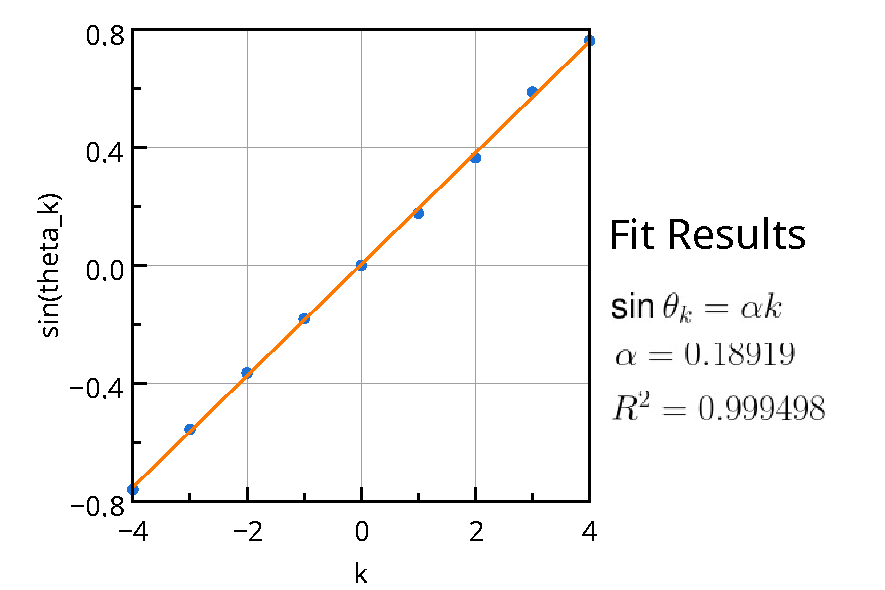
\includegraphics{plot2.pdf}
\end{figure}

The linear fit of $\sin\theta_k$ versus $k$ yields $\alpha = 0.18919$ and $R^2 = 0.999498$//
\[
\lambda = \alpha d 
= \frac{0.18919}{300}\times10^6
=630.63\,\mathrm{nm}
\]

\subsection*{Errors Analysis}
 The relative error is approximately $7.01\%$.Although the linear fitting yields a high coefficient of determination ($R^2=0.999498$), systematic errors may still exist. Possible sources of error include inaccurate angular readings, imperfect alignment of the spectrometer, and uncertainty in the grating constant.The experimental accuracy could be improved by carefully adjusting the optical system, measuring diffraction angles on both sides, and repeating the measurements.

\subsection*{Review Question}
Ensure that the spectrometer is stable and properly maintained\\
Avoid disterbing the optical component after adjusting \\
Read both vernier scales to reduce eccentricity errors
\end{document}